\documentclass{novel}
\usepackage{wrapfig}
\usepackage{lettrine}
\usepackage{changepage}
\usepackage{float}
\usepackage{adjustbox}
\usepackage[round]{natbib} 

\lang      {english}
\title     {}
\subtitle  {}
\authors   {}
\cover     {resources/novel_front.jpg}{resources/novel_back.jpg}
\license   {CC}{by-nc-sa}{4.0}
\isbn      {ECS661U}
\publisher {210517307 \& 210543960}
\edition   {1}{2024}
\dedicate  {Queen Mary University of London}{User Experience Design}
\thank     {Coursework 1}
\keywords  {fiction, template, packages}

\note{This report explores the relationship between technology and London's libraries. As the modern world of computers and smartphones intertwine with the traditional practise of reading, our findings are aptly presented in the classic format of a book.}

\blurb{"Technology in England’s Libraries" explores the effects of devices on user experience. This ethnographic study examines how technology and noise levels affect one another, with data taken from the historic British Library to the modest Lewsey Library. By observing real-world interactions, our research reveals how technology influences learning, social interaction, and personal comfort. \\ \\ Furthermore, this book proposes an innovative new design, created to enhance the library experience through auditory, visual, and tactile feedback to promote quiet and respectful spaces without imposing on visitors or sacrificing collaborative opportunity.}

\begin{document}

\toc

\h{Ethnography}

\hhh{Introduction}
\l{T}his ethnographic study focuses on the effects of technology on user behaviours within different library environments, examining their effects on the user experience of others. Libraries are essential resources for learning and research, providing spaces that contribute significantly to the productivity and comfort levels of many users. The aim of this research is to understand how various elements within library settings, such as device usage, room size, and noise levels, interact to create distinct user experiences.

The study was conducted in eight diverse libraries, ranging from large public libraries in the heart of London, such as the British Library, to Luton's humble Lewsey Library. For a complete list, please refer to the data chapter. These libraries were selected for their varied sizes and the diverse communities they serve. Each location was observed once, providing a snapshot of typical user behaviour and interaction with the environment at different times.

By examining the interplay between space, noise, and technology, we can gain a better understanding of the ideal conditions for different types of library users and how libraries can adapt to meet their users' needs more effectively.

\noindent
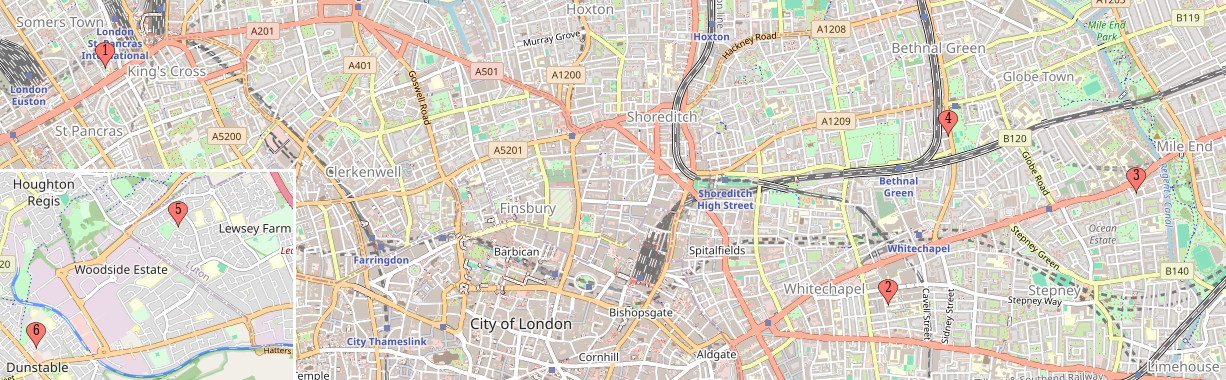
\includegraphics[width=\textwidth]{resources/Map2.png}

\clearpage
\hhh{Findings}
\l{M}ile End Library presents a scenario where technology facilitates social interaction and a sense of community among students. However, this comes at the cost of individual concentration and quiet study. Here, laptop usage was notably higher. In one scenario, a group of four students sharing their exam results led to periods of raised voices and laughter. This interaction highlights how technology can distract people from their surroundings. While for some, this behaviour may create memorable moments that alleviate academic pressure and encourage friendships and communal learning, for others, it may distract from urgent work and increase stress. This incident presents the challenge of maintaining moderate noise levels in spaces while still encouraging collaboration and communication.

\begin{wrapfigure}{r}{0.31\textwidth} 
\vspace{-\intextsep}
    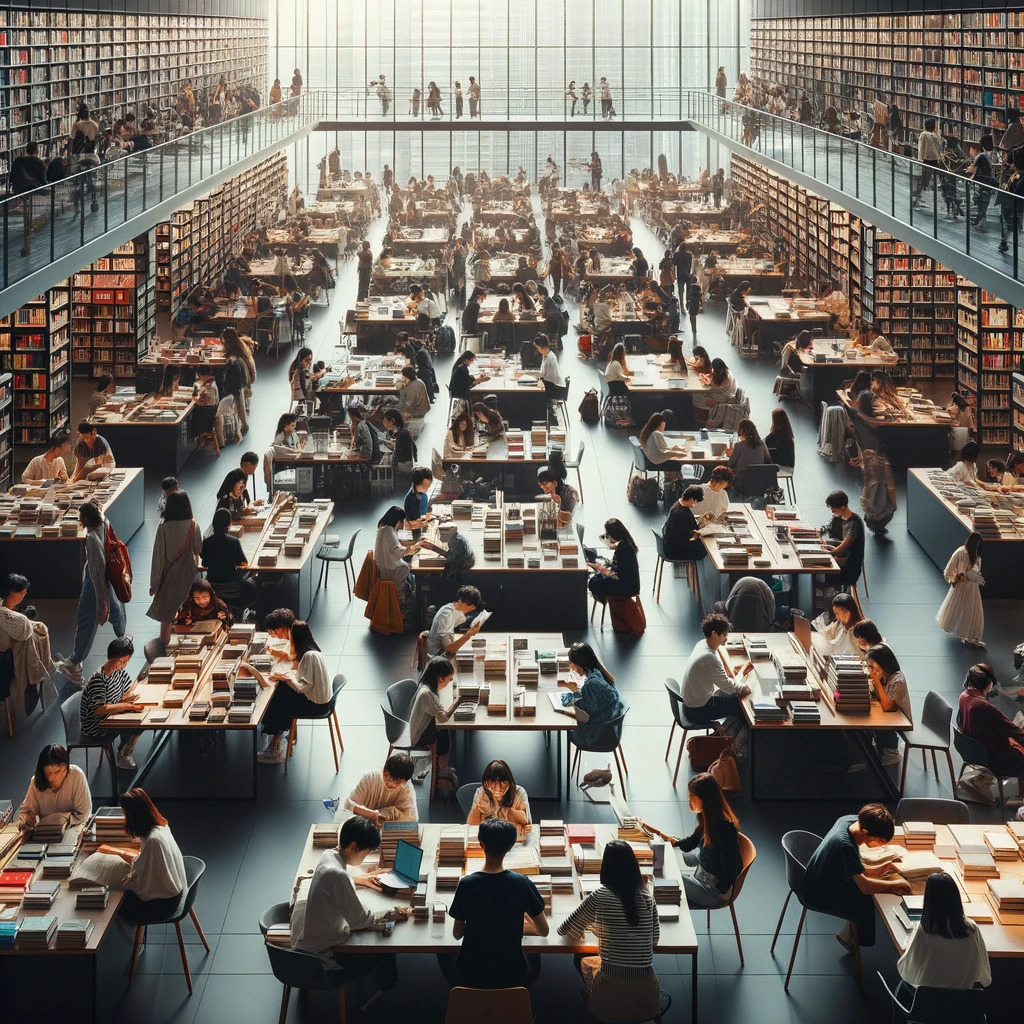
\includegraphics[width=0.31\textwidth]{resources/mileEnd.jpg}
    \vspace{-20pt} % Adjust this value as needed to reduce the gap below the image
\end{wrapfigure}

Unfortunately, for those seeking a quieter space, silent areas are not a significant improvement. In Mile End Library's quiet area, three individuals, focused on their laptops, were observed discussing a group project. Shared content on their screens led them to gradually escalate beyond whispering levels. This breach of quiet room etiquette was not due to malice but rather to the nature of their collaborative work and the insulating effect of laptop screens, which can create a false sense of privacy.

To our surprise, we found that factors such as requiring ID had no substantial impact on noise levels. The general public appear to behave just as appropriately, if not more so, than those with exclusive access. The lack of public computers in the main area of the British Library suggests that surveillance is too challenging in such large areas. This situation mirrors the dynamics of noise regulation, where although the majority can be relied on to maintain silence, a handful of exceptions can disrupt the experience for all.

\begin{wrapfigure}{l}{0.31\textwidth} 
\vspace{-\intextsep}
    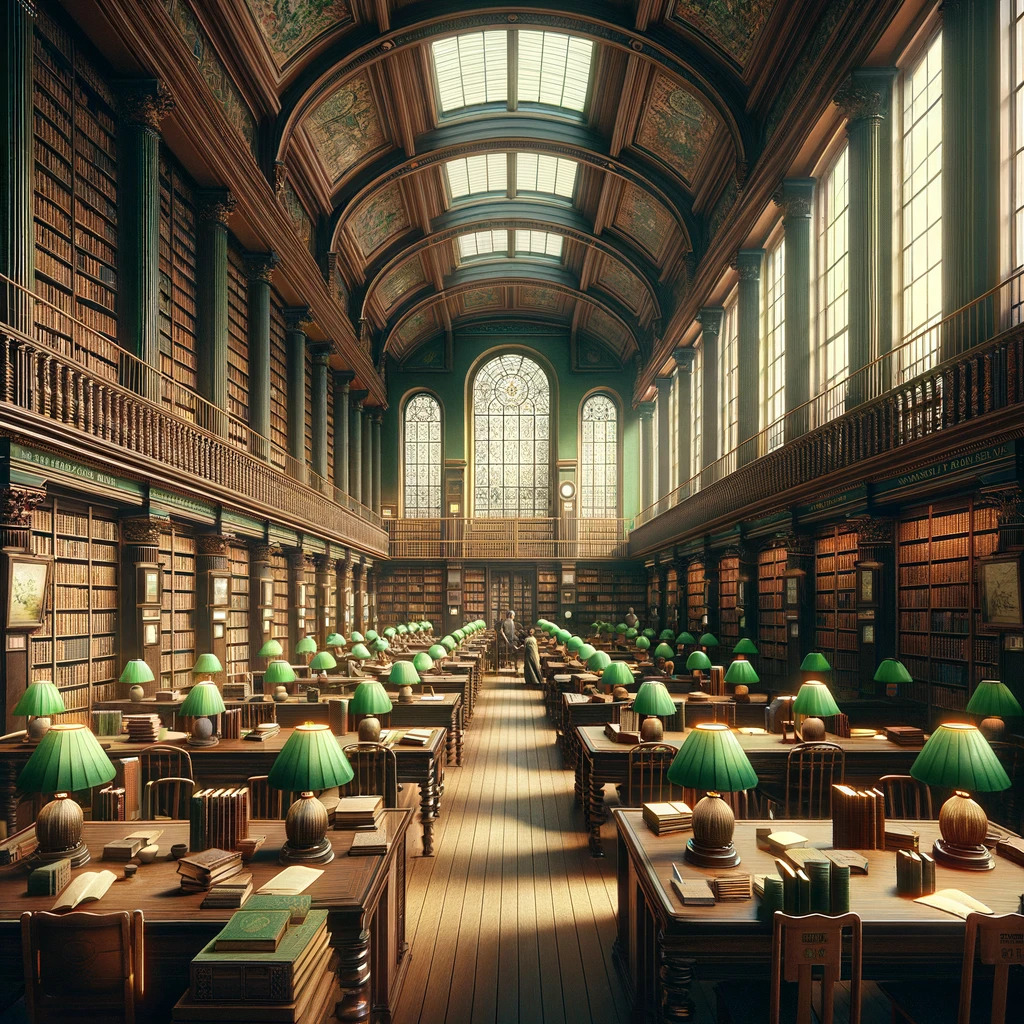
\includegraphics[width=0.31\textwidth]{resources/whitechapel.jpg}
    \vspace{-20pt} % Adjust this value as needed to reduce the gap below the image
\end{wrapfigure}
Despite the British Library Membership Room requiring paid access, and Whitechapel Library being free for students, they showed very different levels of vocal interaction. The British Library Membership Room had four individuals engaging in conversation, Whitechapel Library had none. This variation is likely due to their difference in architectural design; Whitechapel Library's tall ceiling causes echo, encouraging visitors to maintain silence, or risk their voices being heard across the entire building. Being a church in its past, visitors likely still treat it as such. Conversely, Mile End Library, with its very large room size, had significant amounts of loud and moderate conversations, likely due to the perception of anonymity in larger spaces, and the reduced impact of noise on immediate surroundings. Considering the British Library Membership predominantly attracts older, fee-paying clients, rather than young students who enter with just their student IDs, it becomes evident that demographics alone do not dictate noise levels.

\begin{wrapfigure}{r}{0.31\textwidth} 
\vspace{-\intextsep}
    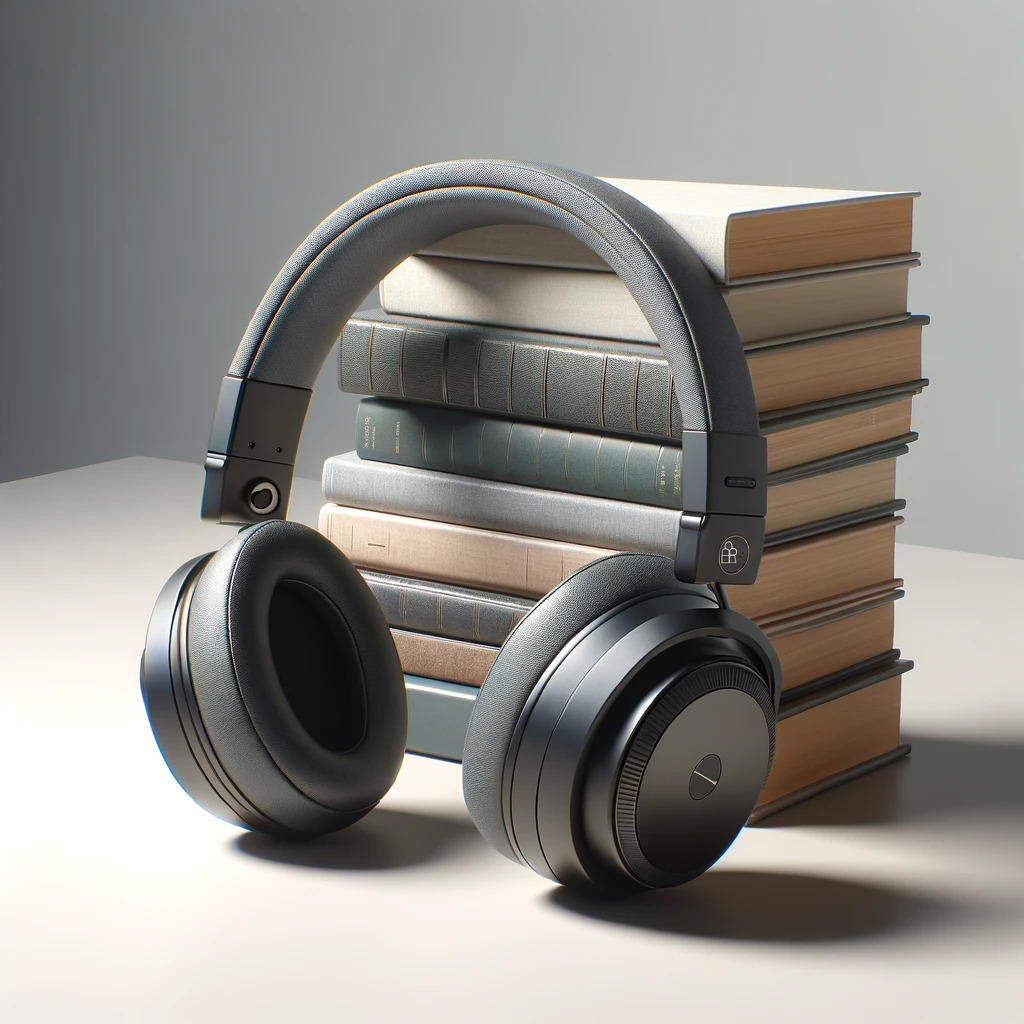
\includegraphics[width=0.31\textwidth]{resources/headphones.jpg}
    \vspace{-20pt} % Adjust this value as needed to reduce the gap below the image
\end{wrapfigure}
In Bethnal Green Library and Whitechapel Library, the advent of noise-cancelling headphones further allows individuals to experience private spaces within a public setting. Most were immersed in their own worlds, isolating themselves from potential distractions. Furthermore, at Whitechapel Library, despite a notable number of individuals on mobile phones, the environment remained quiet. This indicates respectful phone usage that does not disturb others, and reflects social conformance influenced by the library's architectural design. In contrast, at Bethnal Green, an employee had a prolonged conversation with a visitor without the use of any devices. Additionally, Lewsey Library had no reported phone usage, yet two people were talking loudly. This suggests that technology is not the only factor influencing noise levels, and in many cases, it can be seen to decrease noise levels. Social dynamics and the enforcement of library policies likely play a much more significant role.

Moving out of London, Luton's Lewsey Library was the smallest room we observed, yet it had one of the highest noise levels recorded, matching our findings from some other small-room libraries such as the British Library Membership Room. Small rooms tend to amplify minor noises, which can either encourage silence or intensify even moderate conversations. Although the library offers computers, laptops were preferred. Concentration followed the pattern we expected: students are more focused when studying in smaller rooms with fewer people. 

\begin{wrapfigure}{l}{0.30\textwidth} 
\vspace{-\intextsep}
    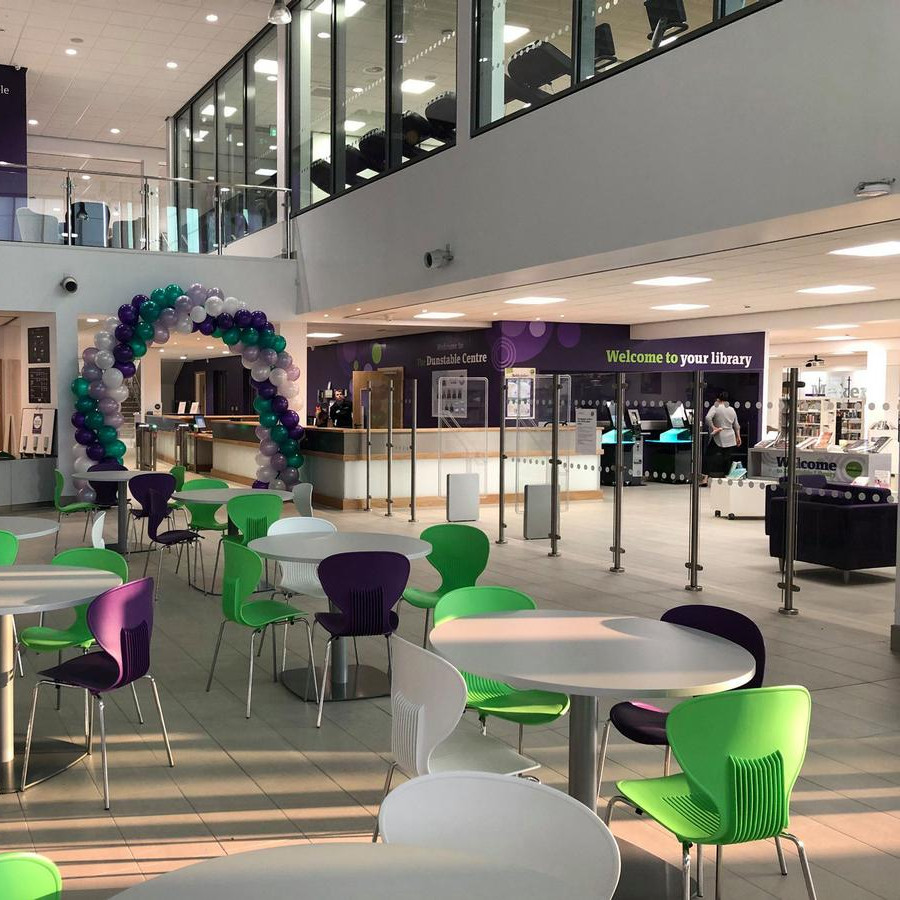
\includegraphics[width=0.30\textwidth]{resources/dunstable.jpg}
\vspace*{-10mm}
    \caption*{{\scriptsize (Tom Walker, 2019)}}
\end{wrapfigure}
On the other hand, Dunstable Library is a moderately large, modern building. Surprisingly, there were few people using mobile or laptop devices; instead, more people seemed to be grouped together working at tables. There were moderate conversation levels between groups, but due to the large open space, it felt fairly quiet overall. Being a modern library, many computers were available and, unlike at Lewsey Library, they were often utilised. This demonstrates how newer equipment is significantly more likely to be used.

\hhh{Literature}
\l{T}he presence of technology in itself does not inherently lead to increased noise levels; rather, it is how and which devices are used, and the surrounding social context that determine the volume. For instance, individuals using laptops with headphones typically maintain a quiet environment, aligning with the expected silence in library settings, as noted by \cite{aarts_silence_2003}. However, when technology is used by groups for collaborative purposes, it tends to raise the overall noise, thereby establishing a new, noisier norm within the library environment. Our findings highlight the complex interaction between technology, environmental cues, and social norms, demonstrating how both identical technology and social groups can result in extremely varying noise levels. This wide range of factors that contribute to noise levels suggests the need for a universal solution to the issue.

\begin{wrapfigure}{l}{0.31\textwidth} 
\vspace{-\intextsep}
    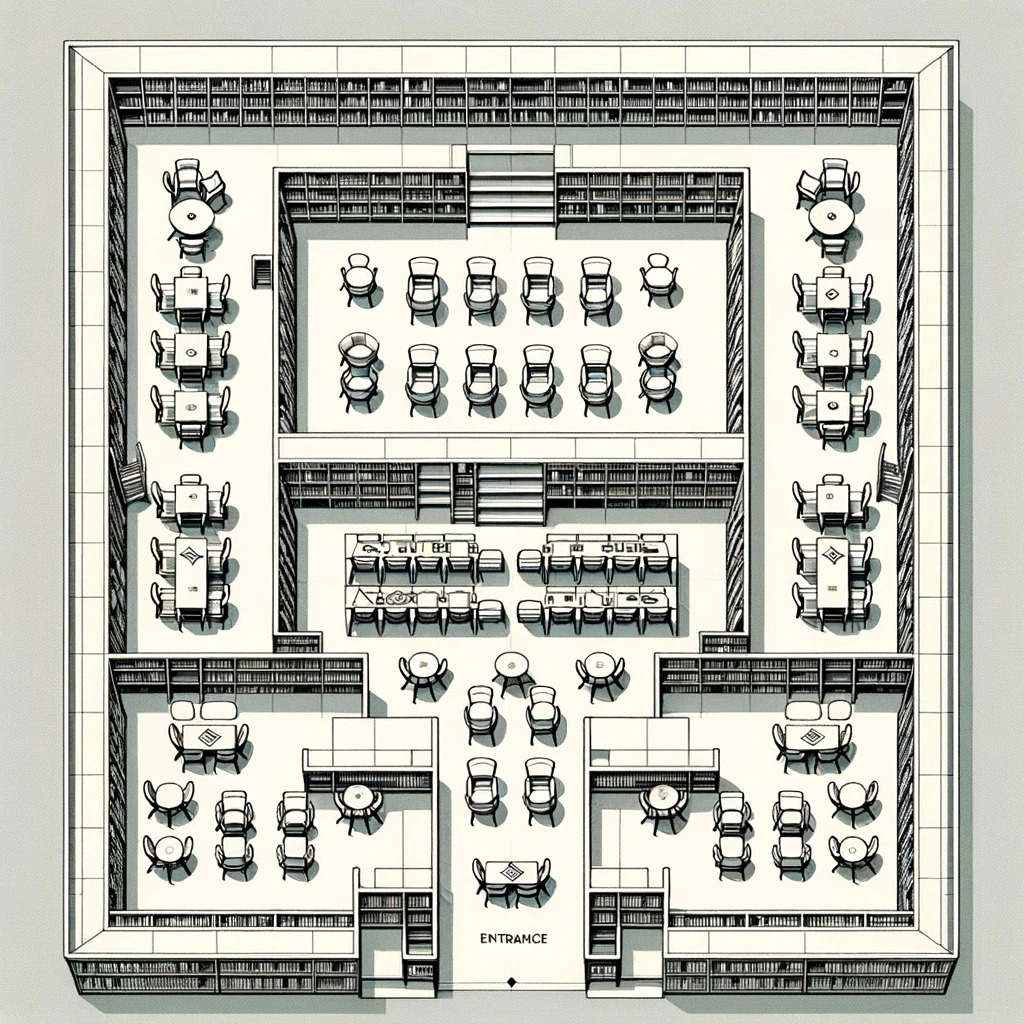
\includegraphics[width=0.31\textwidth]{resources/chairs.jpg}
    \vspace{-20pt} % Adjust this value as needed to reduce the gap below the image
\end{wrapfigure}
However, \cite{luyben_reducing_1981} found that rearranging furniture did not result in significant changes in decibel levels. The most that could be achieved was a reduction in people's own 'subject noise level.' In these cases, the room overall felt quieter when tables and chairs were spread out and facing away from each other. However, this study demonstrates the limited options libraries have for reducing noise using traditional methods. Even if there were significant decibel changes, almost all of the libraries we visited had limited options for seating orientation due to their floor plans. Traditional methods, such as soundproofing and strict librarians, can only do so much; it is likely that a digital solution is required to better control noise levels.

\hhh{Interviews}
\l{B}y being aware of our plan to design a device aimed at decreasing the noise levels in libraries, we recognized the irony in conducting interviews on their premises. Instead, we opted to gather insights from friends about their personal experiences. Although this approach might yield less reliable data, as it is subject to the individuals' recollections, it helps counteract the personal bias we have when collecting the data ourselves. Our initial questions were broad and open-ended to prevent leading the respondents towards specific answers. These questions gradually became more focused, drawing exclusively on the respondents’ earlier responses to pinpoint their specific views and needs.

Person A highlighted the critical need for silent areas, criticising Mile End Library for its distracting environment. They preferred the ITL, as they have the ability to choose from several rooms to find one with the fewest and quietest people. When asked if they had ever confronted someone about their noise levels, they said that they had not but wished they had the courage to do so. On the other hand, Person B stated that they depended on the ability to discuss ideas with their friends in libraries, especially since their course had a large number of group modules. Although they acknowledged that a noisy atmosphere could impair others' concentration, they did not find it to be a significant issue for themselves.

Fortunately, Person A and B have access to various study spaces across campus. The scenario is different for non-students like Person C, who sees libraries as an escape from a noisy home environment. However, despite the significant membership fee, the British Library Membership room did not prove quiet enough for them. Despite these varied opinions, all three interviewees agreed on the necessity of libraries accommodating group work; however, two of them expressed a desperate need for improved noise control measures.

\newgeometry{bottom=0cm, right=4cm, left=4cm, top=3.6cm} % Set the bottom margin as needed
\h{Design}
\l{L}ibrary noise levels are influenced by a range of factors. We can take advantage of the Three Paradigms of Human-Computer Interaction \citep{steve_harrison_three_2007} by creating a system to control room volume. In alignment with the Engineering Paradigm, we can enhance functionality and usability by integrating visual, tactile, and auditory feedback mechanisms into our device. For example, when noise levels exceed the maximum threshold for a prolonged period, a small hidden speaker emits a gentle, non-intrusive sound reminder, while the visual display changes colours. Tactile feedback is provided through the desks with integrated vibration alerts, subtle enough to catch attention without causing disturbance. This multimodal approach ensures that the system accommodates different learning and interaction preferences, and draws from the Information Processing Paradigm by focusing on and understanding human cognitive functions. This not only supports individuals with various sensory preferences and needs but also gives the system multiple routes by which to catch the attention of overly loud visitors. We also know from \cite{marshall_rethinking_2011} that most users assume all public displays support only tapping rather than dragging. Therefore, it makes sense to design a UI that can achieve all tasks without requiring multiple fingers or prolonged motions on the screen. These approaches ensure that all users, including those with disabilities, can receive and understand noise level information. This creates an environment that encourages everyone to control and be conscious of the ambient noise around them, completing the third and final Paradigm of Phenomenology.
\noindent
\begin{figure}[H]
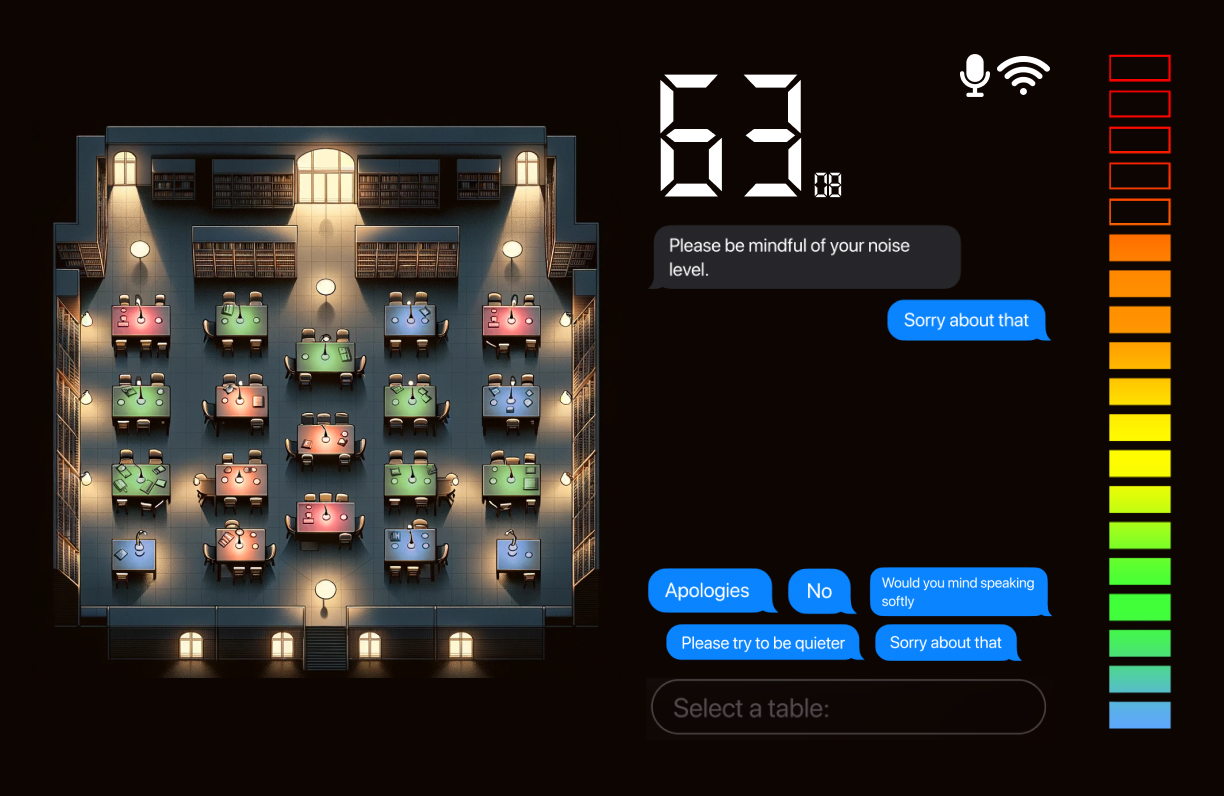
\includegraphics[width=\textwidth]{resources/design.jpg}
\end{figure}
\restoregeometry

The device promotes collective responsibility toward maintaining a conducive work environment. Inspired by theories of social proof \citep{cialdini_influence_2001}, when individuals observe others modifying their behaviour based on the displayed noise levels, they are likely to follow suit. By including an algorithm to alert users that they are much louder than the average desk, we can pressure outliers to reduce their noise levels, thereby decreasing distractions for others. This is also important because each library will have a different base level of noise; therefore, using the same decibel level on every device will not prove effective. The device uses this algorithm to light up desks in orange or red on the top-down map of the library, allowing users to send polite, anonymous messages to problematic desks. This creates a social governance model where users collectively contribute to maintaining an efficient and peaceful environment. This approach is supported by the theory of social translucence by \cite{erickson_social_2000}, which advocates for systems that support cooperative behaviours by making social cues visible and understandable. In a worst-case scenario, where noise is significantly above a predetermined level, staff or security can be notified to visit or view the desk on CCTV. This will increase safety in libraries, and users who are aware of this feature can use it to call for help in emergencies.

\begin{wrapfigure}{r}{0.31\textwidth}
\vspace{-\intextsep}
    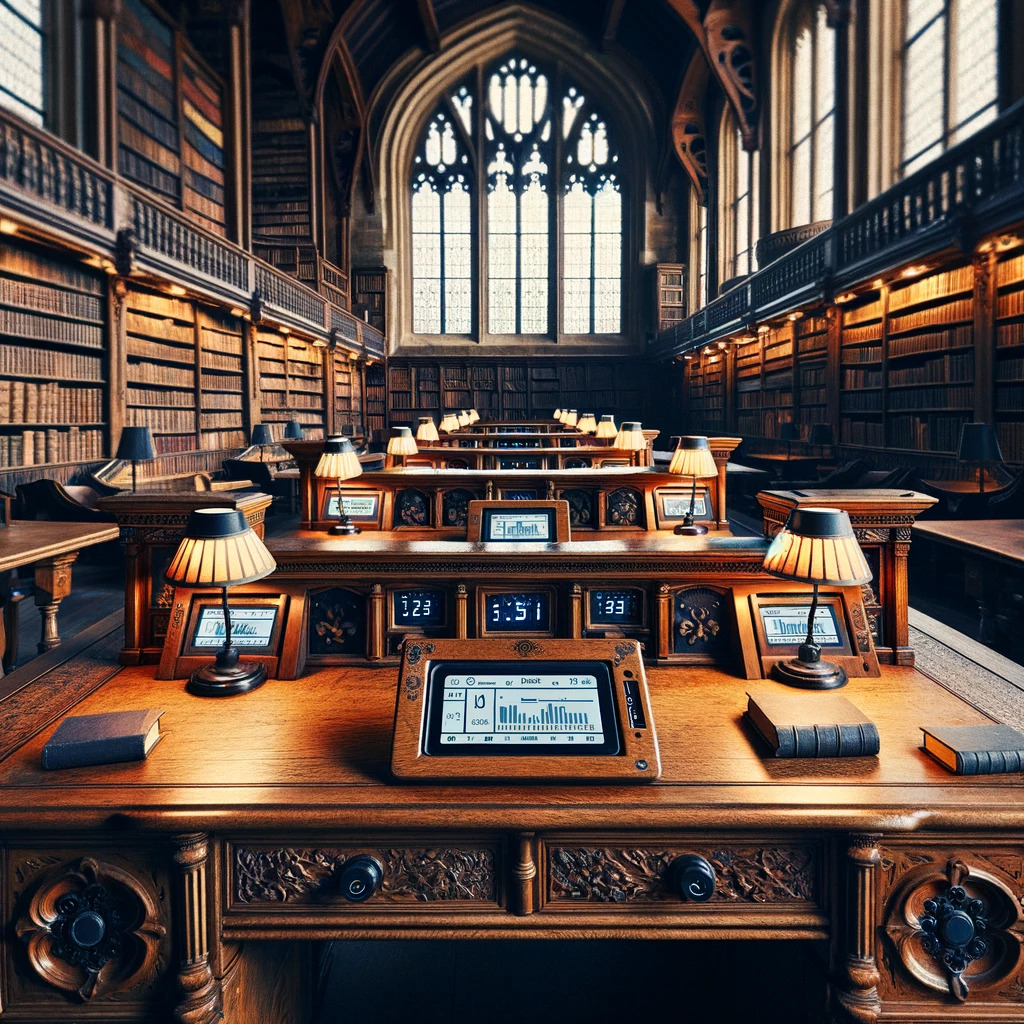
\includegraphics[width=0.31\textwidth]{resources/deskDevice.jpg}
    \vspace{-20pt} % Adjust this value as needed to reduce the gap below the image
\end{wrapfigure}
The design not only serves a functional purpose, but also contributes to the library's ambiance. Drawing on principles from calm technology \citep{denning_coming_1997}, the design is unobtrusive, blending with the library's aesthetics by integrating small screens into desks. Colours and patterns are chosen based on research in colour psychology, with pastel blues and greens representing acceptable noise levels and bright reds indicating higher noise levels that should be avoided \citep{elliot_color_2007}. The tables on the map and the volume metre use these colours to quickly visualise problematic areas. The default dark mode in the UI reduces light pollution in the library, and decibel counters appear as segmented displays. Additionally, all UI elements update only once a second, aligning with the familiar rhythm of a clock, which should help make the display less distracting. As observed in Dunstable Library, modern and aesthetically pleasing equipment is more likely to be utilised and respected. 

Noise level data is processed locally without recording specific sounds or conversations, and communication between desks is anonymized. Respecting user privacy is crucial for fostering trust and acceptance of interactive systems. By ensuring that data is processed locally and interactions remain anonymous, our design adheres to the privacy-by-design principles outlined by \cite{cavoukian_privacy_2010}. If these principles are not adhered to and data is leaked, users are extremely likely to cease attending libraries altogether. The recent cyber-attack on the British Library has already convinced the public that even libraries are not safe from malicious hacking \citep{sir_roly_keating_learning_2024}. In any case, a microphone indicator is always displayed to alert users that their voices are being captured. Since the devices are anonymous and can be used by anyone sitting at the tables, the messages are predetermined. \cite{kraut_internet_2002} and \cite{joinson_self-esteem_2004} highlight the dangers of social interaction with technology and the importance of restricting users to inoffensive texts. By including multiple options, we ensure there is enough content for users to communicate any necessary messages. Users are limited to one text every minute unless there is a reply, and there is a report button to inform library staff of misbehaving individuals.

Rewards such as virtual leaves can be collected for maintaining a quiet environment. These can be exchanged for real-world rewards, leveraging the psychological impact of rewards and aligning with the principles of motivational design. For libraries without the financial capabilities, the display can instead feature a tranquil forest that becomes more animated as noise levels decrease. This provides a subtle distraction that encourages noise reduction without breaking concentration, while promoting noise control in a positive and motivating way. These examples of gamification \citep{deterding_game_2011} make maintaining silence a rewarding experience.

\h{Analysis}
\hhh{Norman's Principles}
\l{N}ormans' first principle is to strengthen visibility of the interface, feedback, and relevant information, allowing users to quickly get the gist of controls \citep{norman_design_1988}. As we have no previous model to analyse, we will be examining our design. Users will notice the left half of the screen shows the library tables surrounding the user, the UI uses "soothing" pastel colours to indicate different noise levels \citep{clark_house_2003}. The distinguishable colours enhance clarity, making it visible even from a distance, the graduation from red to blue displays a spectrum from loudness to quietness. The colour red, a universal signal for attention/caution naturally indicating where high noise levels are, conversely blue is associated with calmness and tranquillity \citep{fipps_psychology_2003}. These colours are not only used to distinct information but leverage intuitive associations to further improve visibility.

Around 50\% of phone users in the UK have an iPhone \citep{kunsts_iphone_2024}; the communication option leverages users' experience with the iPhone's SMS messaging. With similarities in the interface, users should recognise the section as a communication service and feel comfortable using it the first time. Unified Theory of Acceptance and Use of Technology (UTAUT) suggests prior experience is a significant factor in technology acceptance, linking experience to performance and effort expectancy from the user. Comfortability here promotes usability, and the overall goal of the messaging service is to encourage communication with other tables, informing them if they are too loud.

The decibel meter and wifi/microphone symbols are prominently displayed, providing clear guidance on what the system is monitoring and if it is connected to the network. The inclusion of the decibel meter provides users immediate feedback on their own noise level, visualising the invisible audio level to the client. This up to date reading helps whoever is present at the desk keep their voice down. 

Natural Mapping is where the system's controls and actions are arranged in a way that corresponds to a user's intuition and expectations from real world experiences; this can be observed within the floor map of the library tables. It directly corresponds to the physical arrangement in the library. Users can easily locate the source of the noise and communicate swiftly by pressing the corresponding table. Clients can also use the layout to dictate where they prefer to sit, they can quickly glance at the map and move seats accordingly. Furthermore the noise level indicator located on the far right is a common vertical level indicator found on many audio devices, the colour coded noise mapping of these indicators should be picked up by users fairly quickly, with the gradient from red to blue intuitively suggesting a spectrum from quiet to loud.

\clearpage
The decibel metre and wifi/microphone symbols are prominently displayed, providing clear guidance on what the system is monitoring and if it is connected to the network. The inclusion of the decibel metre provides users immediate feedback on their own noise level, visualising the invisible audio level to the client. This up to date reading helps whoever is present at the desk keep their voice down. 

Feedback is crucial in Norman's principles providing feedback to users reassuring them their actions had an positive or negative effect in the system. When a user has sent an sms request to a table asking to lower volume, the UI immediately responds with automated messages to reply with, reassuring the table that originally sent the message that their call for quieter surroundings has been registered. Furthermore the user can see the colour ambience on the floor map and also shift colour signalling a non-disruptive confirmation that their request has been tended to. Alongside is the real time noise monitor through the decibel readings and the audio level indicator, providing dynamic, visual feedback, users can watch their sound levels rise and fall, correlating to their own output and encouraging self regulation. 

\hhh{Phenomenology}
\l{B}reakdown used in phenomenology makes reference to any user-system event that deviates from the expected result the user intended for, resulting in a disconnection with the user interface. This event shifts the system from a 'ready-to-hand state' to a 'present-at-hand state'. Depending on the context these events can either be positive or negative outcomes, and aids the users understanding of the system by exposing them to new experiences.

In the 'ready-to-hand' state of phenomenology, users are fully immersed in their activity with their system interaction, doing so seamlessly without a conscious thought about its workings, activity completion feels entirely natural and intuitive to them. On the other hand the 'present-at-hand' state is the condition of a system after it has been obstructed, users can no longer use it transparently. This causes them to become aware of its existence, attending to it directly, in order to identify the cause of the disruption. This state creates a disconnect between the system and the client, as the user is no longer in a seamless, confident state of engagement.

We can identify a scenario of a breakdown invoking the ready-to-hand and present-to-hand system state. Suppose a group of students working together on a group project sit down at a desk and are absorbed within each others conversations, initially the decibel reader is just part of the environment to them (ready-to-hand state), as they are not explicitly aware of it, yet functioning within the expectations of the users. However once the noise level reaches too high it triggers an audible beep and the level indicator turns red to visualise a breakdown of the system (they may also receive a message asking to be quieter), their seamless activity is disturbed and now requires the students attention (present-at-hand). This shift forces students to reflect on their behaviour and respond to the system, transitioning back to 'ready-to-hand' state.

Furthermore a final state 'unready–to-hand' is when the system itself is faulty. Heidegger highlights three variations of this suspended usability, conspicuousness, obtrusiveness, obstinacy \citep{maybe_unready--hand_2019}. Conspicuousness can relate towards a faulty decibel reader, obtrusiveness relating to the device is missing from the desk, and finally obstinacy can be a continuation of noise regardless of feedback from the device, failing to reach its goal of minimal noise.


\chapter{Bibliography}
\renewcommand{\bibsection}{\hhh{\refname}}
\bibliographystyle{plainnat}
\bibliography{bib}

\clearpage

\newgeometry{bottom=0cm, right=4cm, left=4cm, top=6cm} % Set the bottom margin as needed
\hhh{Images}
\noindent
\centering
To avoid distracting others, and to respect the privacy of all visitors, the following images were produced using OpenAI's DALL-E instead of real photography.

\noindent % Prevent indentation at the beginning of the paragraph

\begin{minipage}{0.33\textwidth}
    
\includegraphics[width=1\textwidth]{resources/square.jpg}
\end{minipage}\hfill
\begin{minipage}{0.33\textwidth}
    \centering
    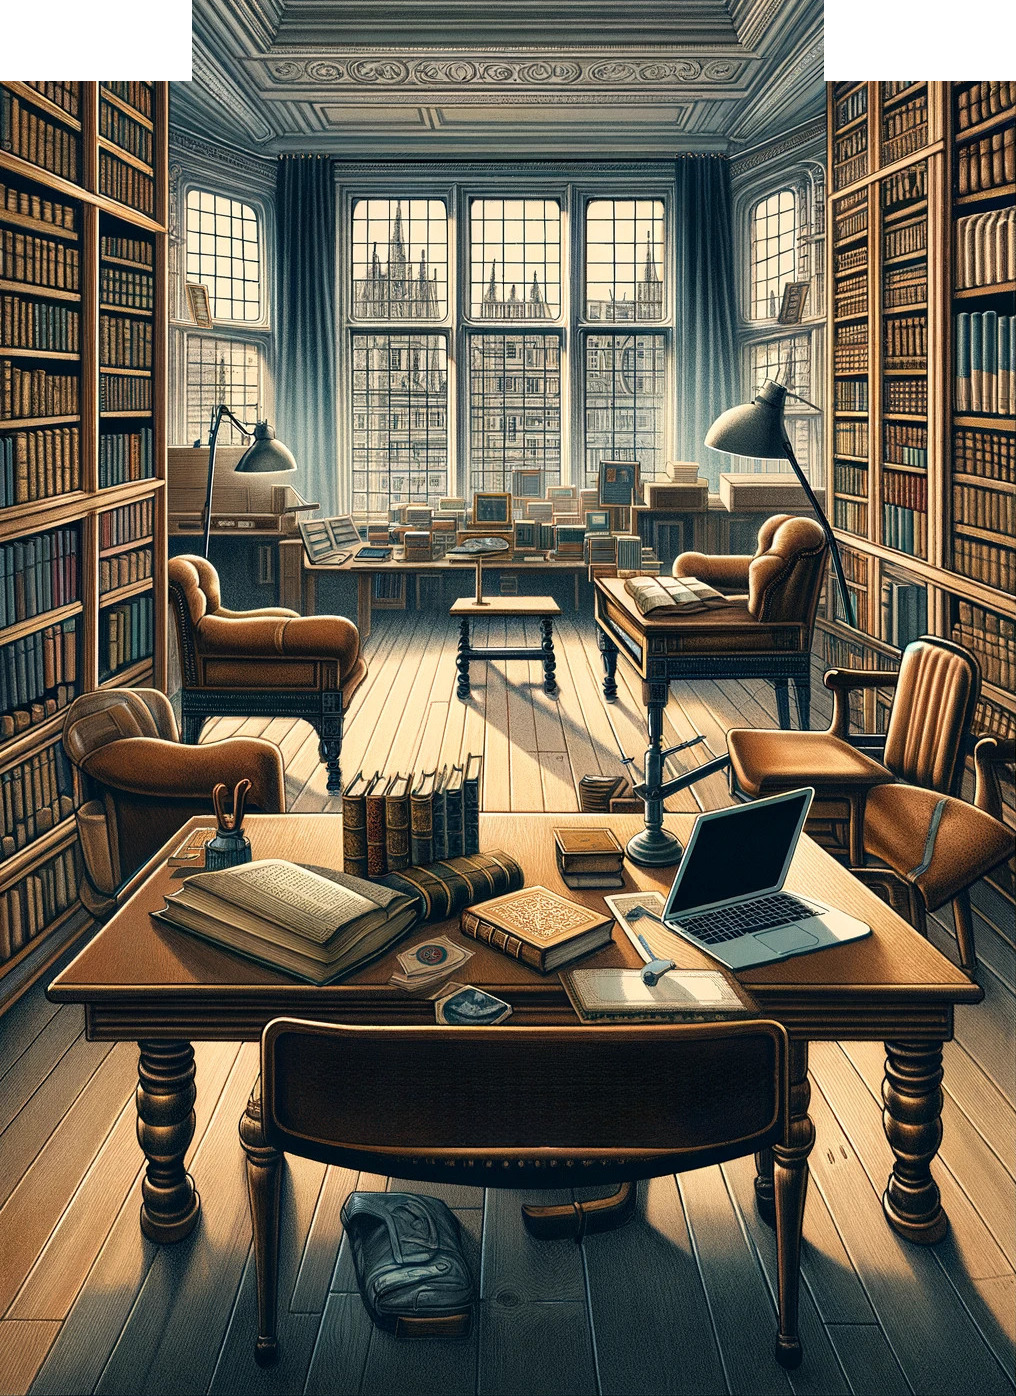
\includegraphics[height=1\textwidth]{resources/novel_front_dalle.jpg}
\end{minipage}\hfill
\begin{minipage}{0.33\textwidth}
    
\includegraphics[width=1\textwidth]{resources/square.jpg}
\end{minipage}\hfill
\begin{minipage}{0.33\textwidth}
    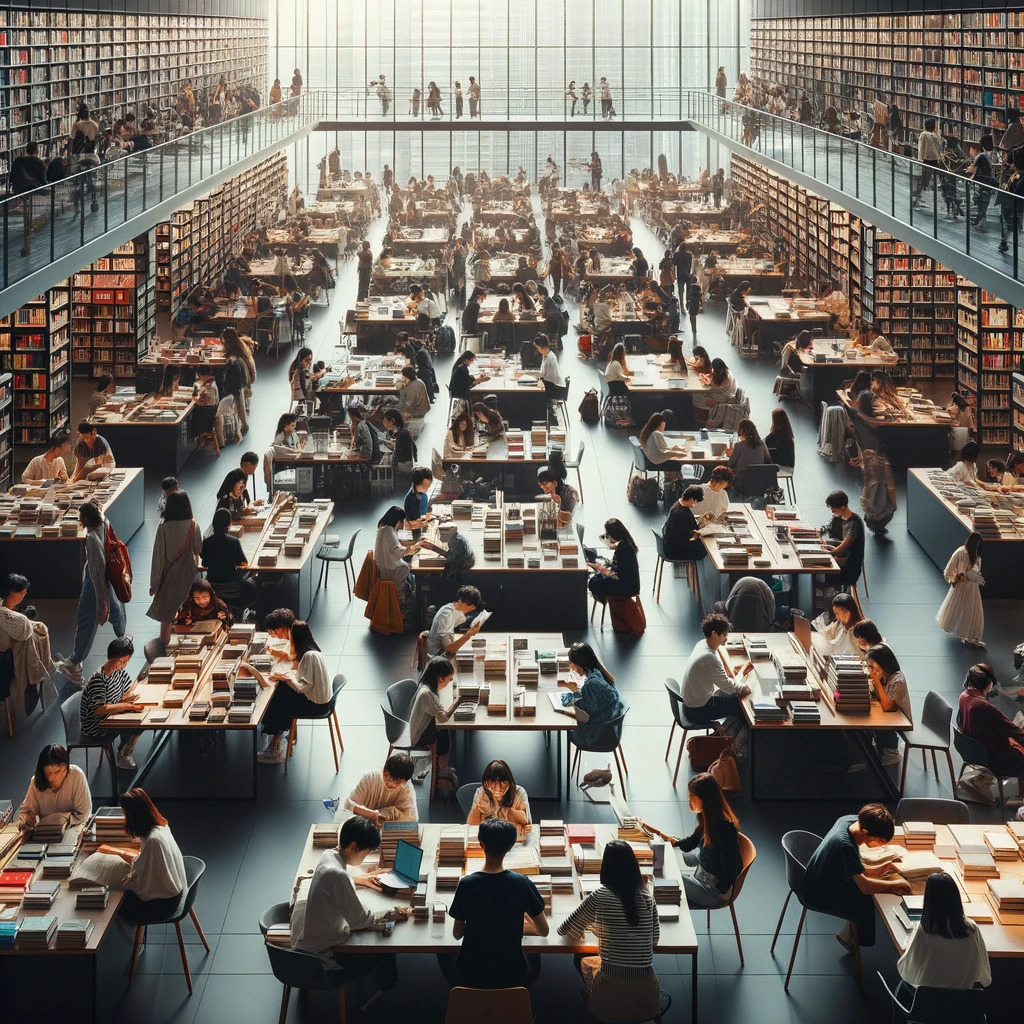
\includegraphics[width=1\textwidth]{resources/mileEnd.jpg}
\end{minipage}\hfill
\begin{minipage}{0.33\textwidth}
    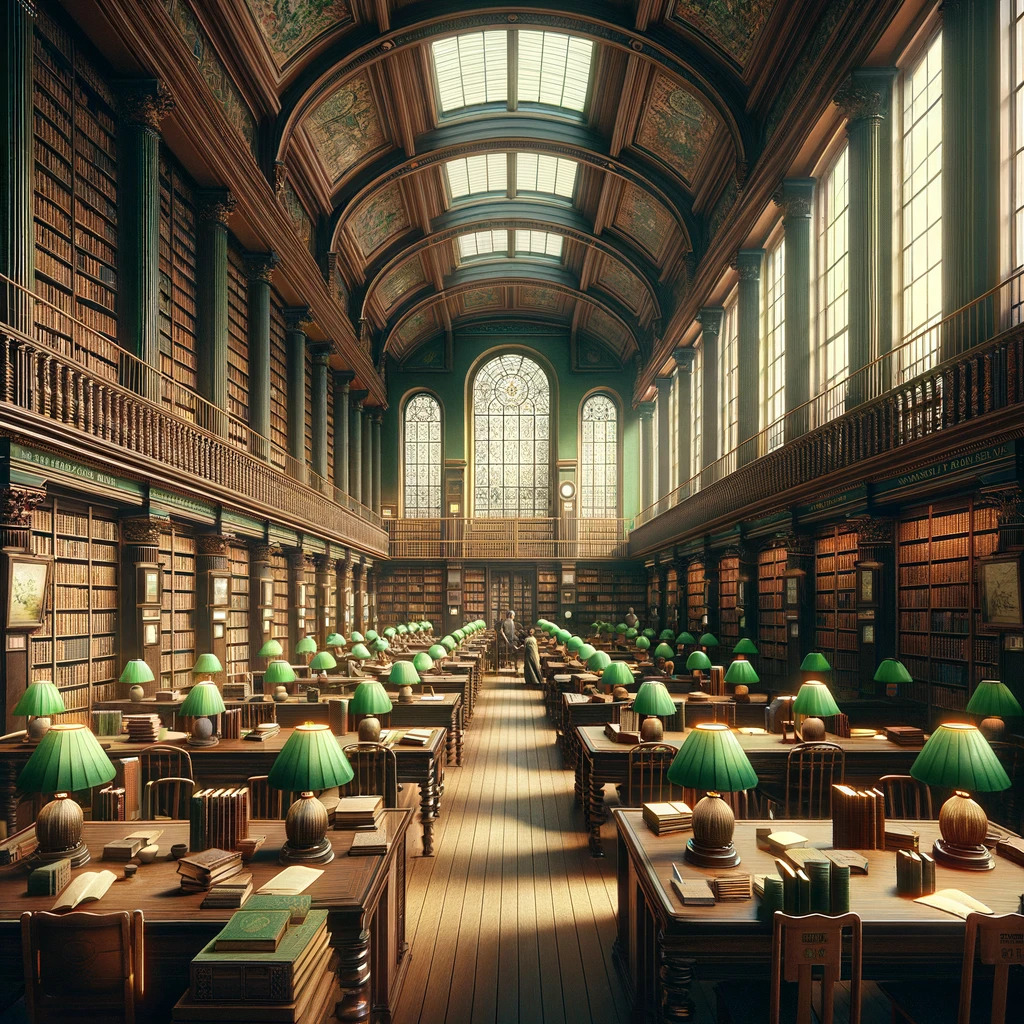
\includegraphics[width=1\textwidth]{resources/whitechapel.jpg}
\end{minipage}
\begin{minipage}{0.33\textwidth}
    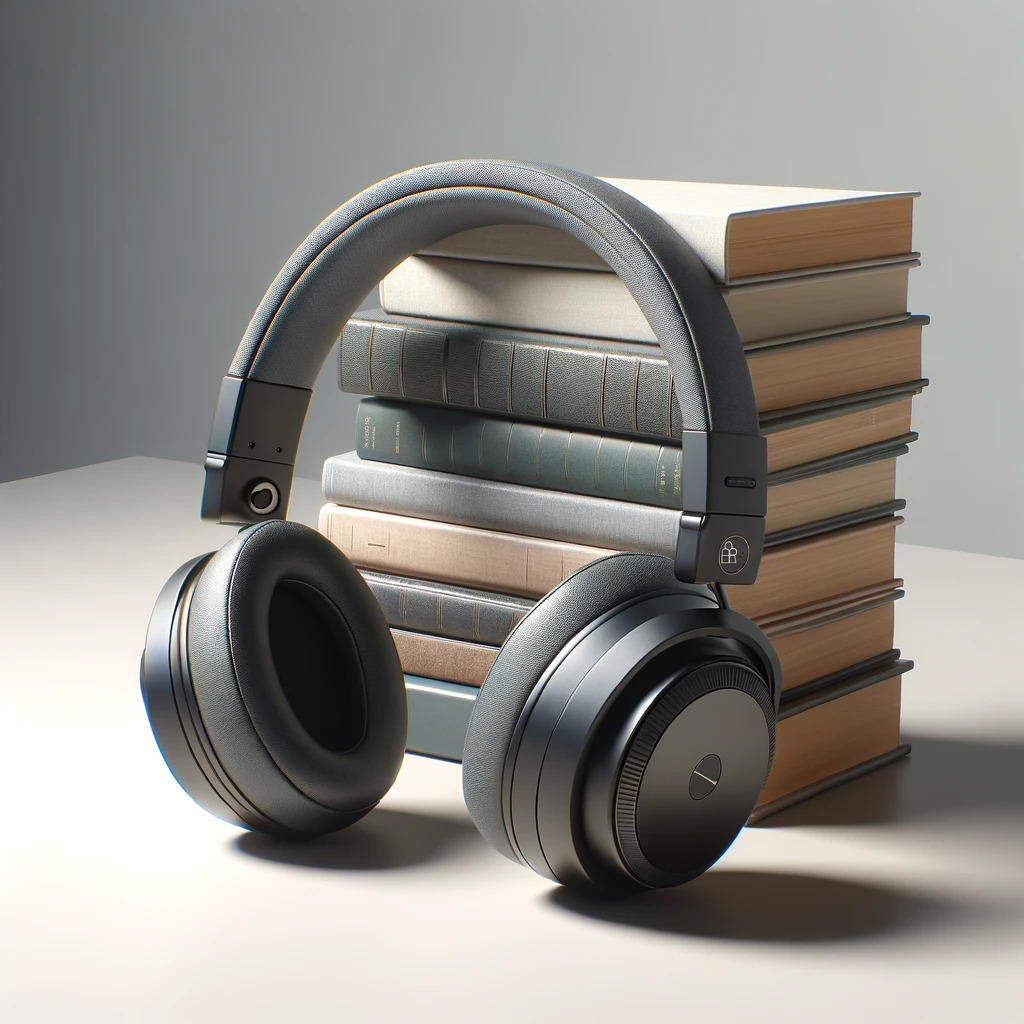
\includegraphics[width=1\textwidth]{resources/headphones.jpg}
\end{minipage}\hfill
\begin{minipage}{0.33\textwidth}
    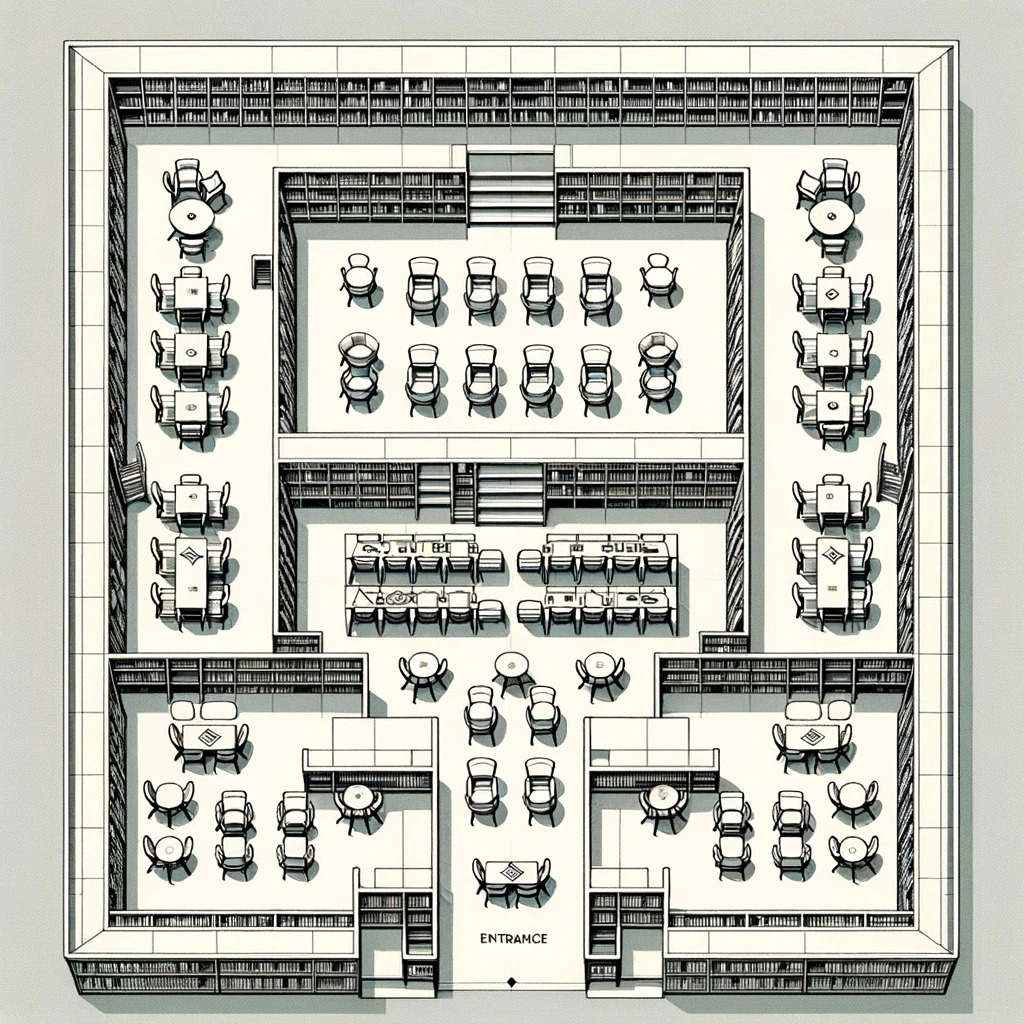
\includegraphics[width=1\textwidth]{resources/chairs.jpg}
\end{minipage}\hfill
\begin{minipage}{0.33\textwidth}
    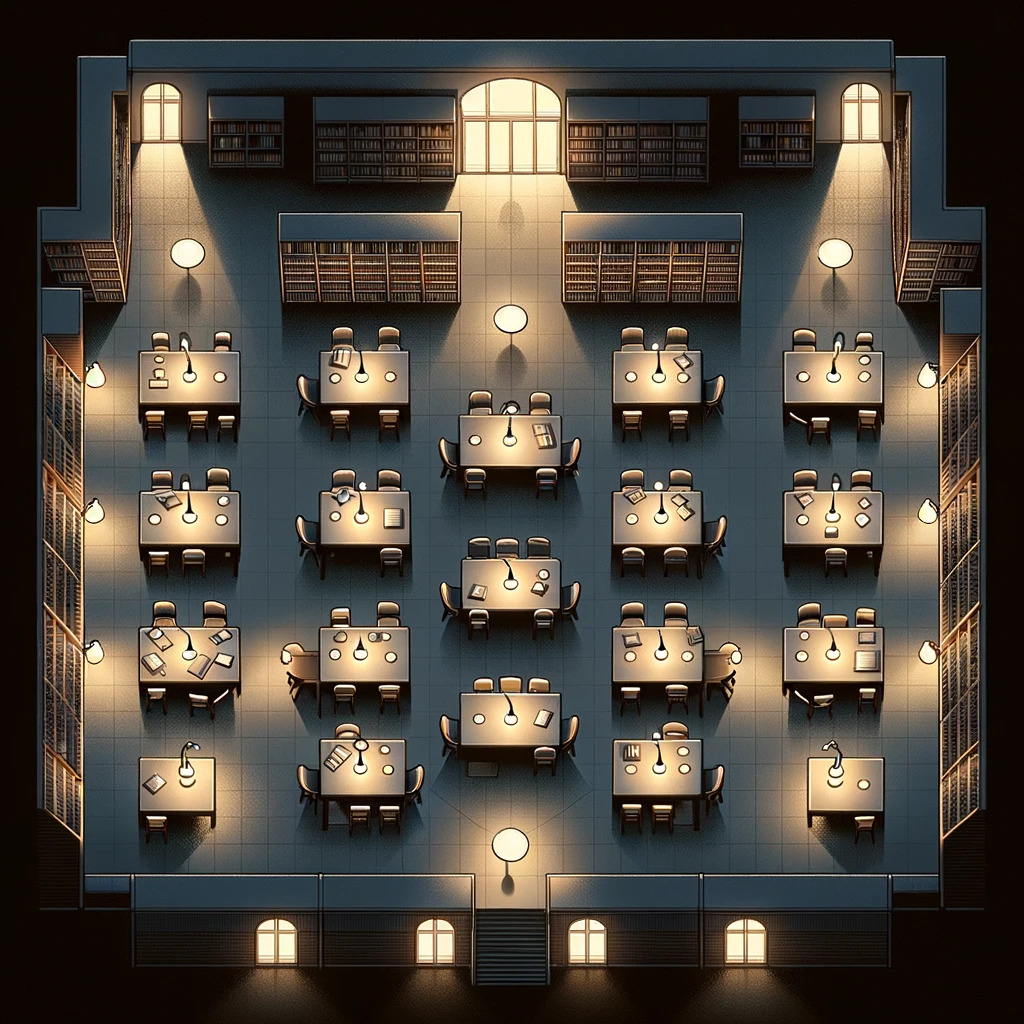
\includegraphics[width=1\textwidth]{resources/designDesks.jpg}
\end{minipage}
\begin{minipage}{0.33\textwidth}
    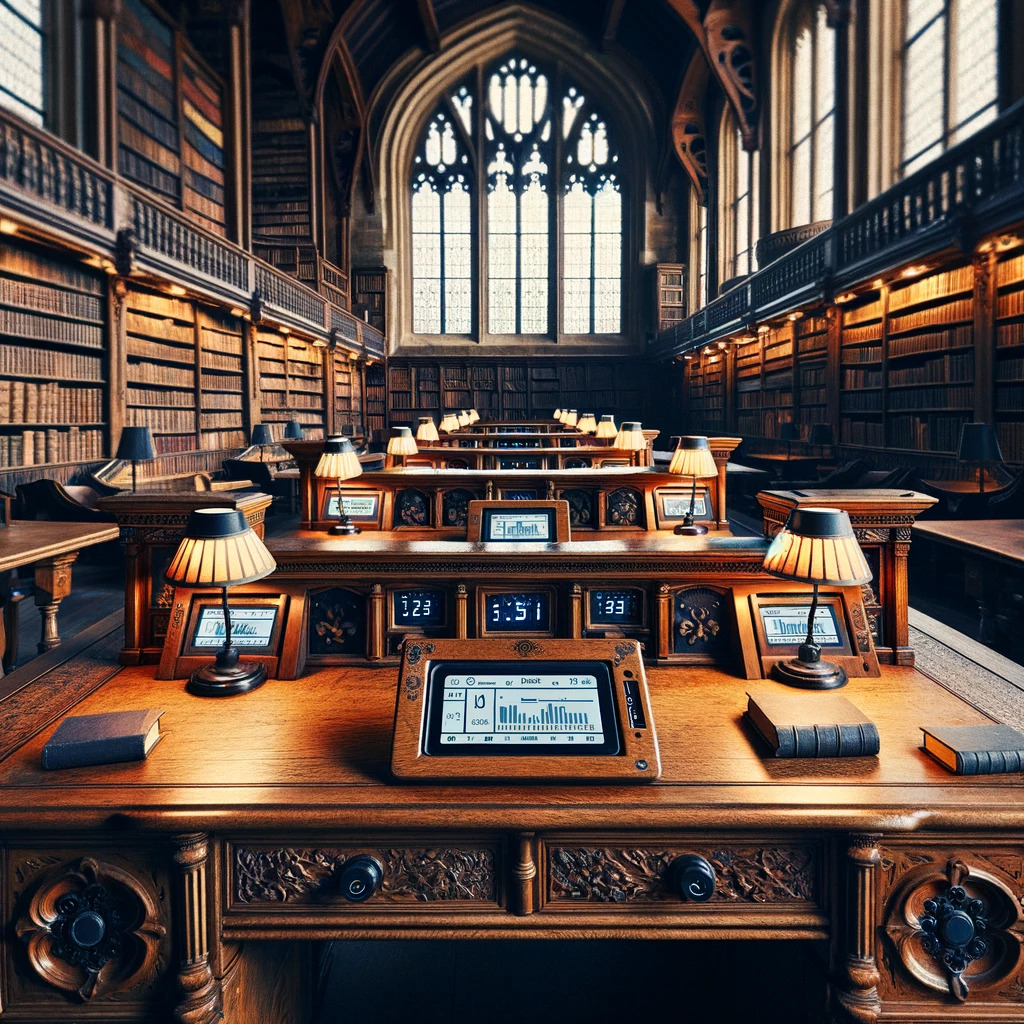
\includegraphics[width=1\textwidth]{resources/deskDevice.jpg}
\end{minipage}
\restoregeometry


\newgeometry{bottom=0cm, right=2cm, left=2cm, top=7cm} % Set the bottom margin as needed
\h{Appendices}
\hhh{Quantitative-Data}
    \centering
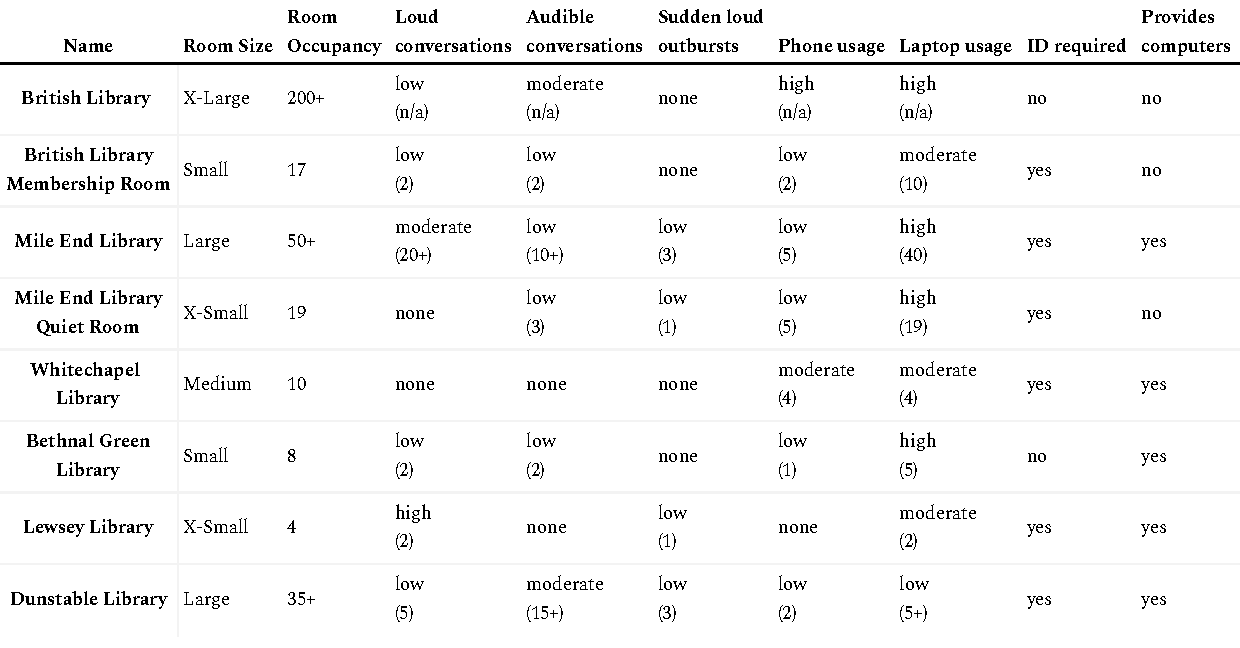
\includegraphics[width=\dimexpr\paperwidth-4cm\relax]{resources/numData.pdf}
\restoregeometry

\newgeometry{bottom=0cm, right=2cm, left=2cm, top=6cm} % Set the bottom margin as needed
\hhh{Qualitative-Data}
    \centering
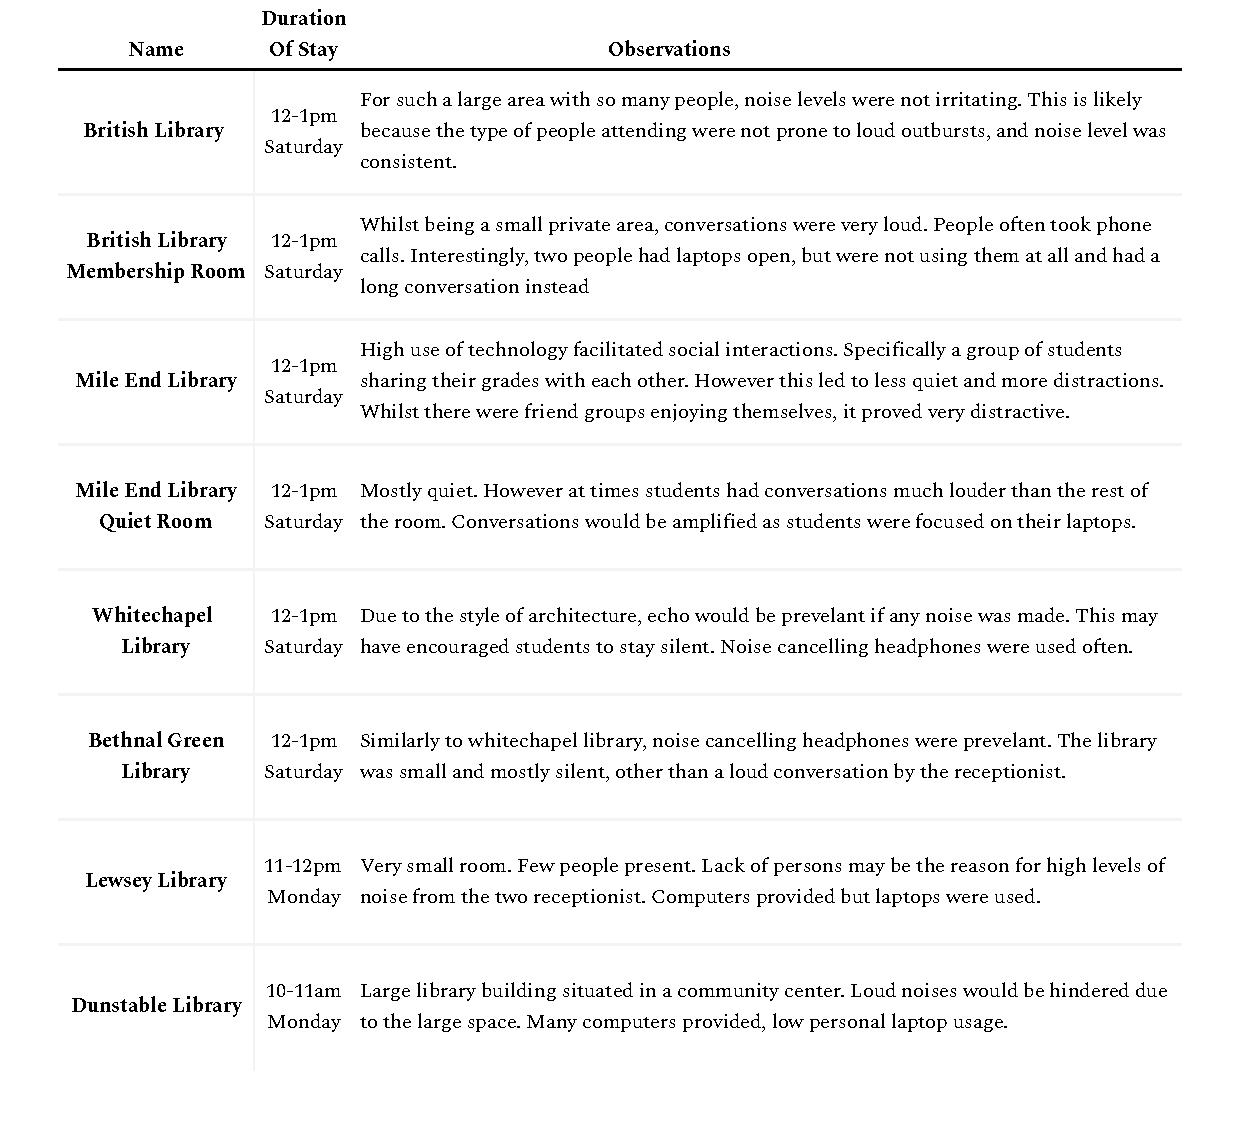
\includegraphics[width=\dimexpr\paperwidth-4cm\relax]{resources/wordData.pdf}
\restoregeometry

\newgeometry{bottom=0cm, right=2cm, left=2cm, top=3cm} % Set the bottom margin as needed
\hhh{Interview-Data}
    \centering
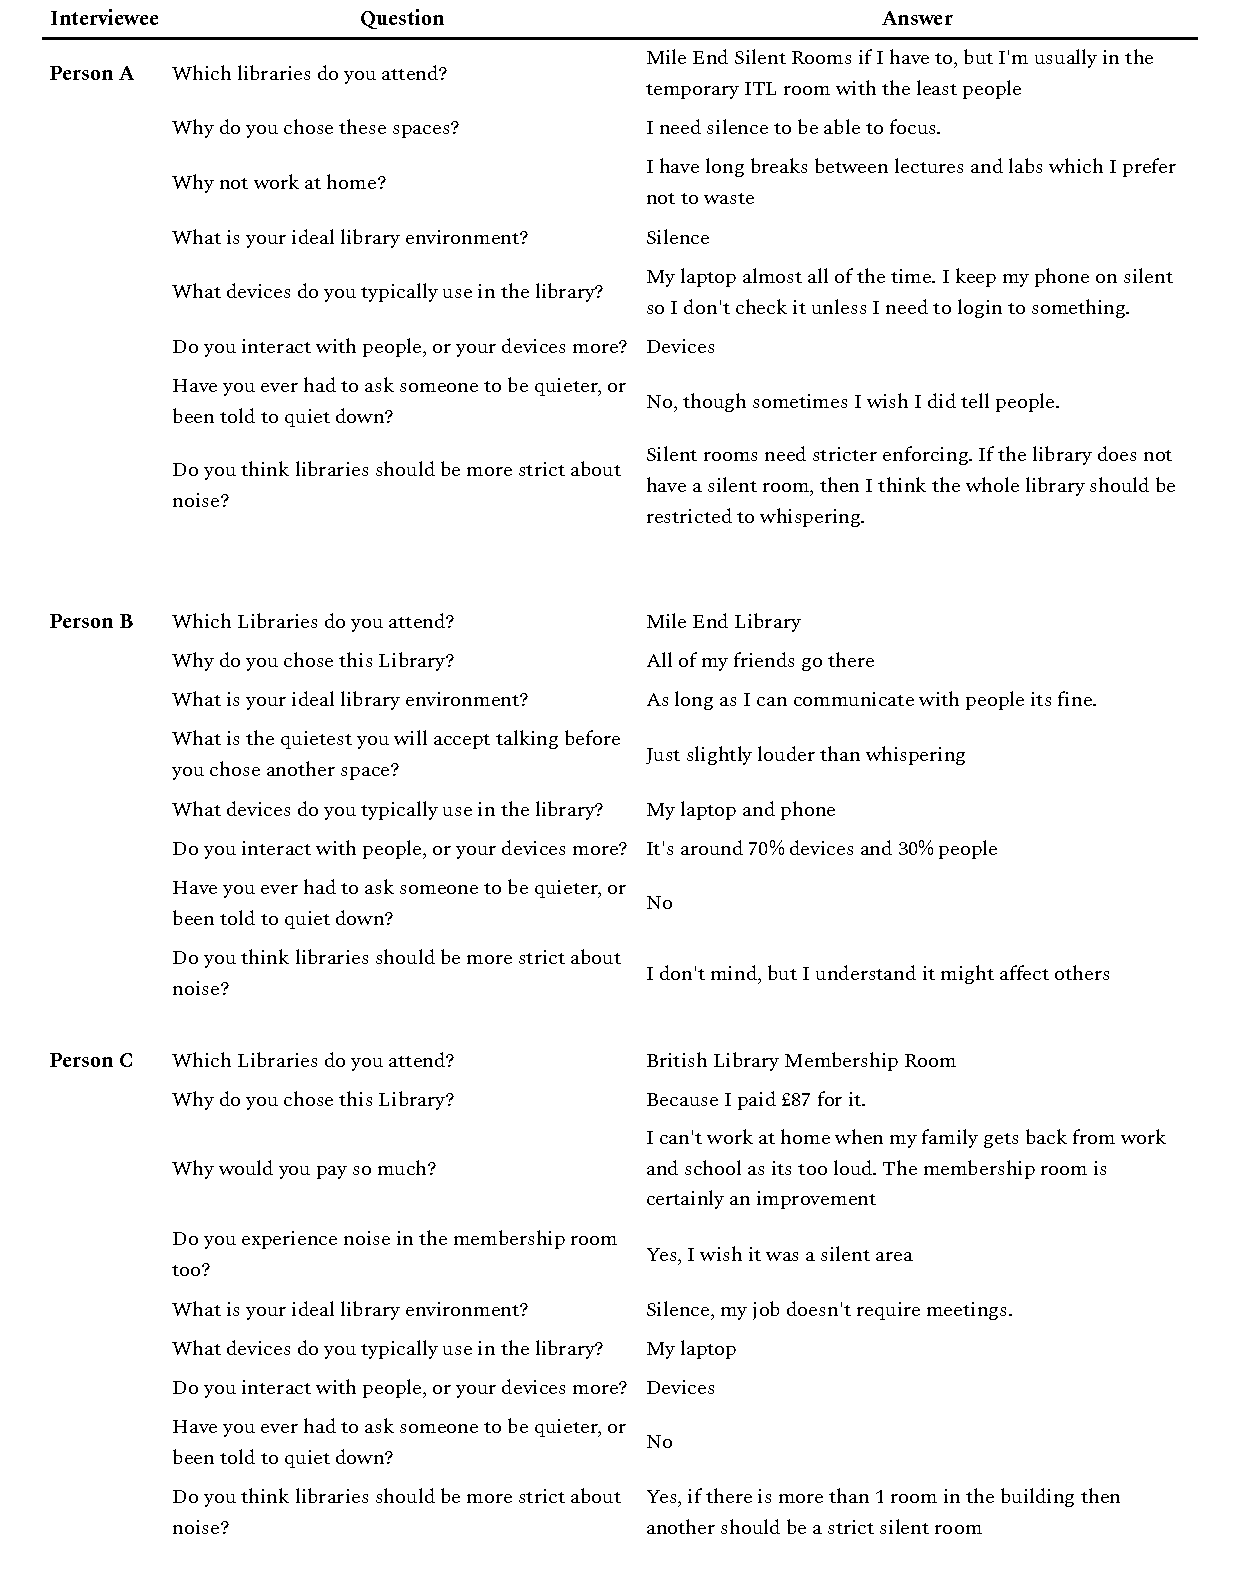
\includegraphics[width=\dimexpr\paperwidth-4cm\relax]{resources/interData.pdf}
\restoregeometry

\end{document}
